\documentclass[tikz, border=10pt]{standalone}
\usepackage{pgfplots}
\usepackage{amsmath}
\usetikzlibrary{backgrounds}
\pgfplotsset{compat=1.18}

\begin{document}
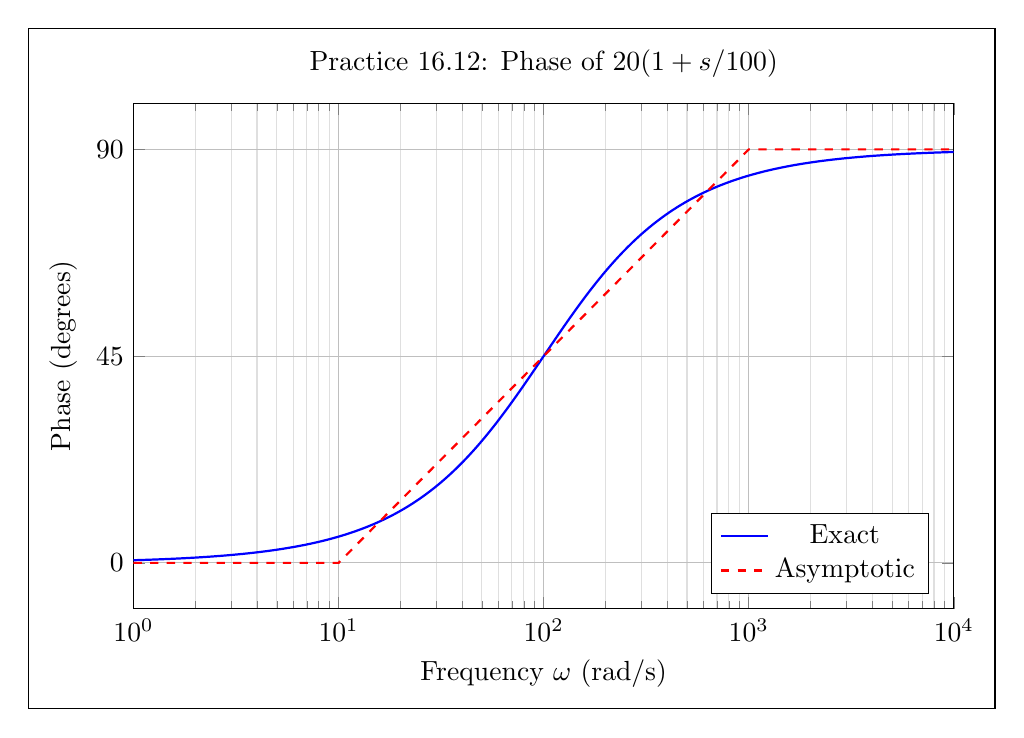
\begin{tikzpicture}[show background rectangle]
    \begin{semilogxaxis}[
        width=12cm, height=8cm,
        title={Practice 16.12: Phase of $20(1 + s/100)$},
        xlabel={Frequency $\omega$ (rad/s)},
        ylabel={Phase (degrees)},
        grid=both,
        xmin=1, xmax=10000,
        ymin=-10, ymax=100,
        minor grid style={gray!25},
        major grid style={gray!50},
        legend pos=south east,
        ytick={0, 45, 90},
    ]

    % Exact: atan(x/100)
    \addplot[blue, thick, domain=1:10000, samples=300] {atan(x/100)};
    \addlegendentry{Exact}

    % Asymptotic
    % Break freq a=100.
    % 0.1a = 10 -> 0 deg
    % 10a = 1000 -> 90 deg
    \addplot[red, dashed, thick] coordinates {
        (1, 0) (10, 0) (1000, 90) (10000, 90)
    };
    \addlegendentry{Asymptotic}
    
    \end{semilogxaxis}
\end{tikzpicture}
\end{document}
